\section{Attestation}
\begin{frame}
    \frametitle{Attestation}
    \begin{itemize}[<+->]
        \item Attestation is used to verify the integrity of an enclave:
        \begin{itemize}[<+->]
            \item Verifies that the code is trustable
            \item That the enclave code has not been tampered with
        \end{itemize}
        \item For attestation a report will be generated by enclave, which contains the identity, measurement of the enclave and a supplied message from other enclave
        \item Report is encrypted by the enclave with a symmetric key between target enclave and processor
        \item Attestation is used to verify integrity of enclaves on same CPU or via remote 
    \end{itemize}
\end{frame}

\begin{frame}
    \frametitle{Local Attestation}
    \begin{columns}
        \begin{column}{0.4\textwidth}
            \begin{enumerate}[<+->]
                \item Enclave A receives the enclave Measure (MRENCLAVE) from enclave B via an established channel
                \item Enclave A generates the report for B with MRENCLAVE and sends the report back so B can verify using EGETKEY
                \item Enclave B generates the report for A with the MRENCLAVE from A and sends it back to get verified from A
            \end{enumerate}
        \end{column}
        \begin{column}{0.6\textwidth}
            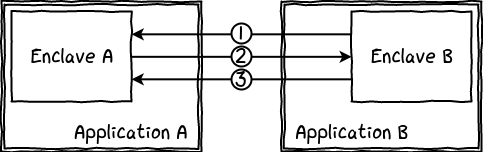
\includegraphics[scale=0.45]{Images/local_attestation.png}
        \end{column}
    \end{columns}
\end{frame}

\begin{frame}
    \frametitle{Remote Attestation}
    \begin{columns}
        \begin{column}{0.4\textwidth}
            \begin{enumerate}[<+->]
                \item Application receives an attestation request from challenger
                \item Application requests report
                \item Application receives report
                \item Report is send to quoting enclave (QE)
                \item QE converts local report to remote report (Quote) and sends back
                \item Challenger receives quote
                \item Attestation verification service verifies quote
            \end{enumerate}
        \end{column}
        \begin{column}{0.6\textwidth}
            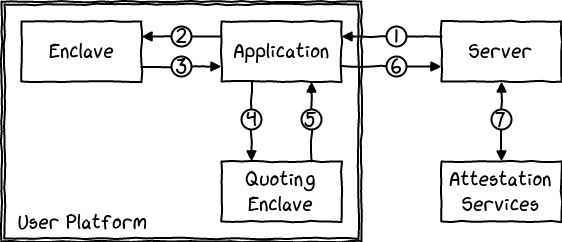
\includegraphics[scale=0.4]{Images/remote_attestation.png}
        \end{column}
    \end{columns}
\end{frame}

\begin{frame}
    \frametitle{Sealing}
    \begin{itemize}[<+->]
        \item Secrets of an enclave gets lost when enclave is closed
        \item Process of encrypting enclave secrets for persistent storage is called sealing
        \item The data can be signed with different keys
        \item Enclave retrieves the sealing key using the EGETKEY instruction, which returns a cryptographic key
        \item Enclaves can seal data with MRENCLAVE as key, so no other enclave is able to read data
        \item Other key is MRSIGNER, so every enclave with same author can read each others data
    \end{itemize}
\end{frame}